\documentclass[10pt,a4paper]{article}
\usepackage[utf8]{inputenc}
\usepackage[margin=1in]{geometry}
\usepackage{titlesec}
\usepackage{booktabs}
\usepackage{titling}
\usepackage{amsmath}
\usepackage{graphicx}
\usepackage{tabularx}
\usepackage{microtype}
\usepackage[hidelinks]{hyperref}

\newcommand{\titlefont}{\bfseries\sffamily\small}
\newcommand{\descfont}{\scriptsize\sffamily\color{black!80}}

% TikZ and its libraries
\usepackage{tikz}
\usetikzlibrary{shapes.geometric, positioning, arrows.meta, calc}

% ALWAYS load hyperref last!
\usepackage{hyperref}
% Custom section formatting
\titleformat{\section}{\large\bfseries}{\thesection}{1em}{}
\titleformat{\subsection}{\normalsize\bfseries}{\thesubsection}{1em}{}

\begin{document}

% ==========================================
% PAGE 1: TITLE PAGE & EXECUTIVE SUMMARY
% ==========================================

\begin{titlepage}
    \pagenumbering{gobble}
    \centering
    \vspace*{1.5cm}

    {\Huge \bfseries RoleTect} \\[0.5cm]
    {\large \bfseries Zero Setup, Lightweight \LaTeX{} IDE \& Privacy-Focused LLM Orchestrated Career Vault} \\[1.5cm]

    \rule{\linewidth}{0.5mm} \\[0.6cm]
    {\large \bfseries Technical Architecture \& Product Case Study} \\[0.2cm]
    \rule{\linewidth}{0.5mm} \\[2.5cm]

    \begin{minipage}{0.45\textwidth}
        \begin{flushleft} \large
            \emph{Author:} \\
            Md. Ramjan Miah \\
            \href{https://github.com/AhmedTrooper/RoleTect}{\textbf{RoleTect} (Source Code)} \\
            {\textbf{\href{https://youtu.be/_imINpqe9mo}{Youtube Intro}}} \\
            Firefox extension \textbf(\href{https://addons.mozilla.org/en-US/firefox/addon/roletect-ingest/}{Click here})
        \end{flushleft}
    \end{minipage}
    \begin{minipage}{0.45\textwidth}
        \begin{flushright} \large
            \emph{Date:} \\
            June 2026
        \end{flushright}
    \end{minipage}

    \vfill




\end{titlepage}




\pagenumbering{arabic}
\setcounter{page}{1}

\clearpage
\section{Executive Summary}
In today's hyper-competitive job market, candidates face a critical paradox: securing interviews requires dynamically tailoring resumes and cover letters to defeat Applicant Tracking Systems (ATS), yet the manual workflow to achieve this is fragmented, exhausting, and insecure. This paper introduces the \textbf{LLM-Orchestrated, Privacy-First, Centralized Job Application Vault}, a fresh paradigm that unifies sovereign user data control with automated document optimization.

Compounding the workflow friction, modern \textbf{researchers and professionals} are bottlenecked by heavy typesetting environments, traditionally requiring bloated \textbf{3-5GB+ local LaTeX distributions} or \textbf{yielding data custody to third-party cloud compilers}. We resolve this dilemma by leveraging the use of a novel \textbf{Local-First, Lightweight LaTeX Compilation Engine}. By \textbf{eliminating heavy dependency overhead, this system slashes local installation footprints from gigabytes to a self-contained, zero-configuration runtime}, ensuring local document compilation occurs entirely client-side to maintain complete data privacy.


\subsection*{The Problem: Workflow Fragmentation \& Security Risks}
\begin{itemize}
    \item \textbf{Operational Fatigue:} Candidates and researchers must navigate a disjointed pipeline of manual text extraction, cloud LLM portals, external \LaTeX{} compilers, and third-party job trackers. This friction causes severe \textbf{workflow bottlenecking}.
    \item \textbf{The \LaTeX{} Bloat Dilemma:} Legitimate document typesetting traditionally forces users to install massive, \textbf{5GB+ local \LaTeX{} distributions}. This heavy overhead discourages adoption and creates immense friction for rapid, iterative document generation.
    \item \textbf{Data Vulnerability:} Centralizing highly granular \textbf{Personally Identifiable Information (PII)} on third-party SaaS platforms exposes users to corporate data monetization, systemic brokering, and \textbf{targeted phishing campaigns}.
\end{itemize}

\subsection{The RoleTect Solution}
\textbf{RoleTect} introduces a definitive shift away from third-party cloud-dependent and resource-heavy utilities. Architected as a cross-platform, \textbf{local-first (cloud extensible)} ecosystem (interactive web extension + Tauri v2 + Axum), it completely centralizes the application lifecycle while ensuring data sovereignty.

We have effectively solved the \LaTeX{} overhead problem by replacing traditional, bloated engines with \textbf{Tectonic}, a \textbf{streamlined, self-contained compilation runtime}. This allows for professional-grade \textbf{document rendering without the multi-gigabyte footprint}. The entire \textbf{operational lifecycle runs entirely on-device/private cloud} to eliminate data privacy risks. Your data never leaves your machine, and your \textbf{API keys} are \textbf{cryptographically} secured using OS-level \textbf{AES encryption}.

\vspace*{2cm}



% =========================================================================
% PAGE 2: PROBLEM STATEMENT & SYSTEMIC INEFFICIENCIES
% =========================================================================
\section{The Deep-Dive Problem Statement}
The modern job application pipeline is fundamentally fractured. To clear technical screeners, candidates must continuously tailor professional documentation to the semantic footprint of each vacancy—introducing an exhausting, multi-platform loop that compromises privacy, organization, and efficiency.

\subsection{The Multi-Platform Friction Loop}
Standard application workflows require manual execution across four disjointed tiers:
\begin{enumerate}
    \item \textbf{Data Ingestion:} Copying unstructured job data from web portals while battling localized copy-blocks and dynamic UI barriers.
    \item \textbf{Context Orchestration:} Pasting payloads into web LLMs and designing custom prompts to execute profile tailoring.
    \item \textbf{Compilation \& Rendering:} Migrating output code to cloud \LaTeX{} clusters (e.g., Overleaf) to debug typesetting \& compile desired document.
    \item \textbf{State Tracking:} Downloading the PDF while \textbf{manually logging metrics} (salaries, dates) into a \textbf{separate dashboard}.
\end{enumerate}
This environment-hopping breaks data continuity. Once a static PDF is downloaded, the link between its compilation state, markup variations, and the source job description is lost, \textbf{making it difficult to match the precise resume variation during a callback}.

\subsection{The Privacy Paradox and PII Exposure}
\textbf{To bypass these bottlenecks, candidates frequently surrender data sovereignty to centralized SaaS platforms.} Hosting comprehensive professional, financial, and educational records on remote cloud clusters triggers critical vulnerabilities:
\begin{itemize}
    \item \textbf{Data Monetization:} Platforms routinely subsidize operations by aggregating, processing, and \textbf{brokering granular candidate profiles to third-party marketing frameworks and recruitment syndicates.}
    \item \textbf{Security Exploitation:} Secondary distribution of Personally Identifiable Information (PII) directly fuels targeted spam, coordinated phishing, fraudulent employment scams, and credential exposure.
\end{itemize}

\subsection{Technical Barriers \& Ecosystem Paywalls}
Existing open-source or self-hosted alternatives present equally steep boundaries. Securing data privacy through \textbf{private deployment requires heavy systems engineering}: \textbf{local Docker} networks, {hosting dense runtimes}, or \textbf{managing local TeX Live environments that exceed 3-5~GB} in disk space. This forces \textbf{non-technical applicants to choose between convenience and privacy}. Furthermore, commercial SaaS providers exploit this gap by \textbf{locking high-fidelity visual assets (e.g., Mermaid.js architecture flowcharts) behind premium subscription} paywalls or \textbf{throttling export resolutions}.


\subsection{Ecosystem Performance Metric Analysis}
RoleTect decouples professional asset production from traditional SaaS platform subscriptions. Table 1 provides an operational breakdown of RoleTect's technical advantages:

\begin{table}[h]
\centering
\caption{System Performance \& Structural Comparison}
\vspace{2mm}
\begin{tabularx}{\textwidth}{>{\raggedright\arraybackslash}p{0.23\textwidth}>{\raggedright\arraybackslash}X>{\raggedright\arraybackslash}X}
\toprule
\textbf{Evaluation Metric} & \textbf{Centralized SaaS (Teal/Overleaf)} & \textbf{RoleTect Ecosystem} \\
\midrule
Monthly Overhead Cost & \$10 -- \$30 / month recurring & \textbf{\$0.00} (Pay-per-token or Free) \\
Privacy Vulnerability & High Risk (PII Cloud Storage) & \textbf{Zero Risk} (OS Keyring / AES-256) \\
Model Independence & Proprietary / Locked-In Vendor & \textbf{Total Freedom} (AWS Bedrock/Ollama local) \\
\textbf{Compilation Latency} & 1 -- 10 Seconds (Network Dependent) & \textbf{Very low} (On-Device Cache) \\
Asset Resolution Limit & Restricted / Paywalled & \textbf{Uncapped} (Up to 16K Vector Exports) \\
\bottomrule
\end{tabularx}
\end{table}

% ==========================================
% PAGE 2: HIGH-COMPLEXITY WORKFLOW & ARCHITECTURE DIAGRAM
% ==========================================
    \vspace{30mm}



\section{System Architecture \& Workflow Blueprint}
The structural interactions between RoleTect's local micro-server data ingress, Vue 3 Pinia state stores, \textbf{dynamic model orchestration, and self-healing LaTeX compilation loops} are mapped systematically below. This diagram explicitly visualizes the \textbf{5 primary AI and systemic workflows} that drive the application's full potential.

\subsection{Architectural Component Specifications}
The vector topology detailed above demonstrates a robust decoupling of structural concerns designed for highly competitive technical validation, explicitly tracking all cross-stack workflows:















\begin{center}
\resizebox{\textwidth}{!}{
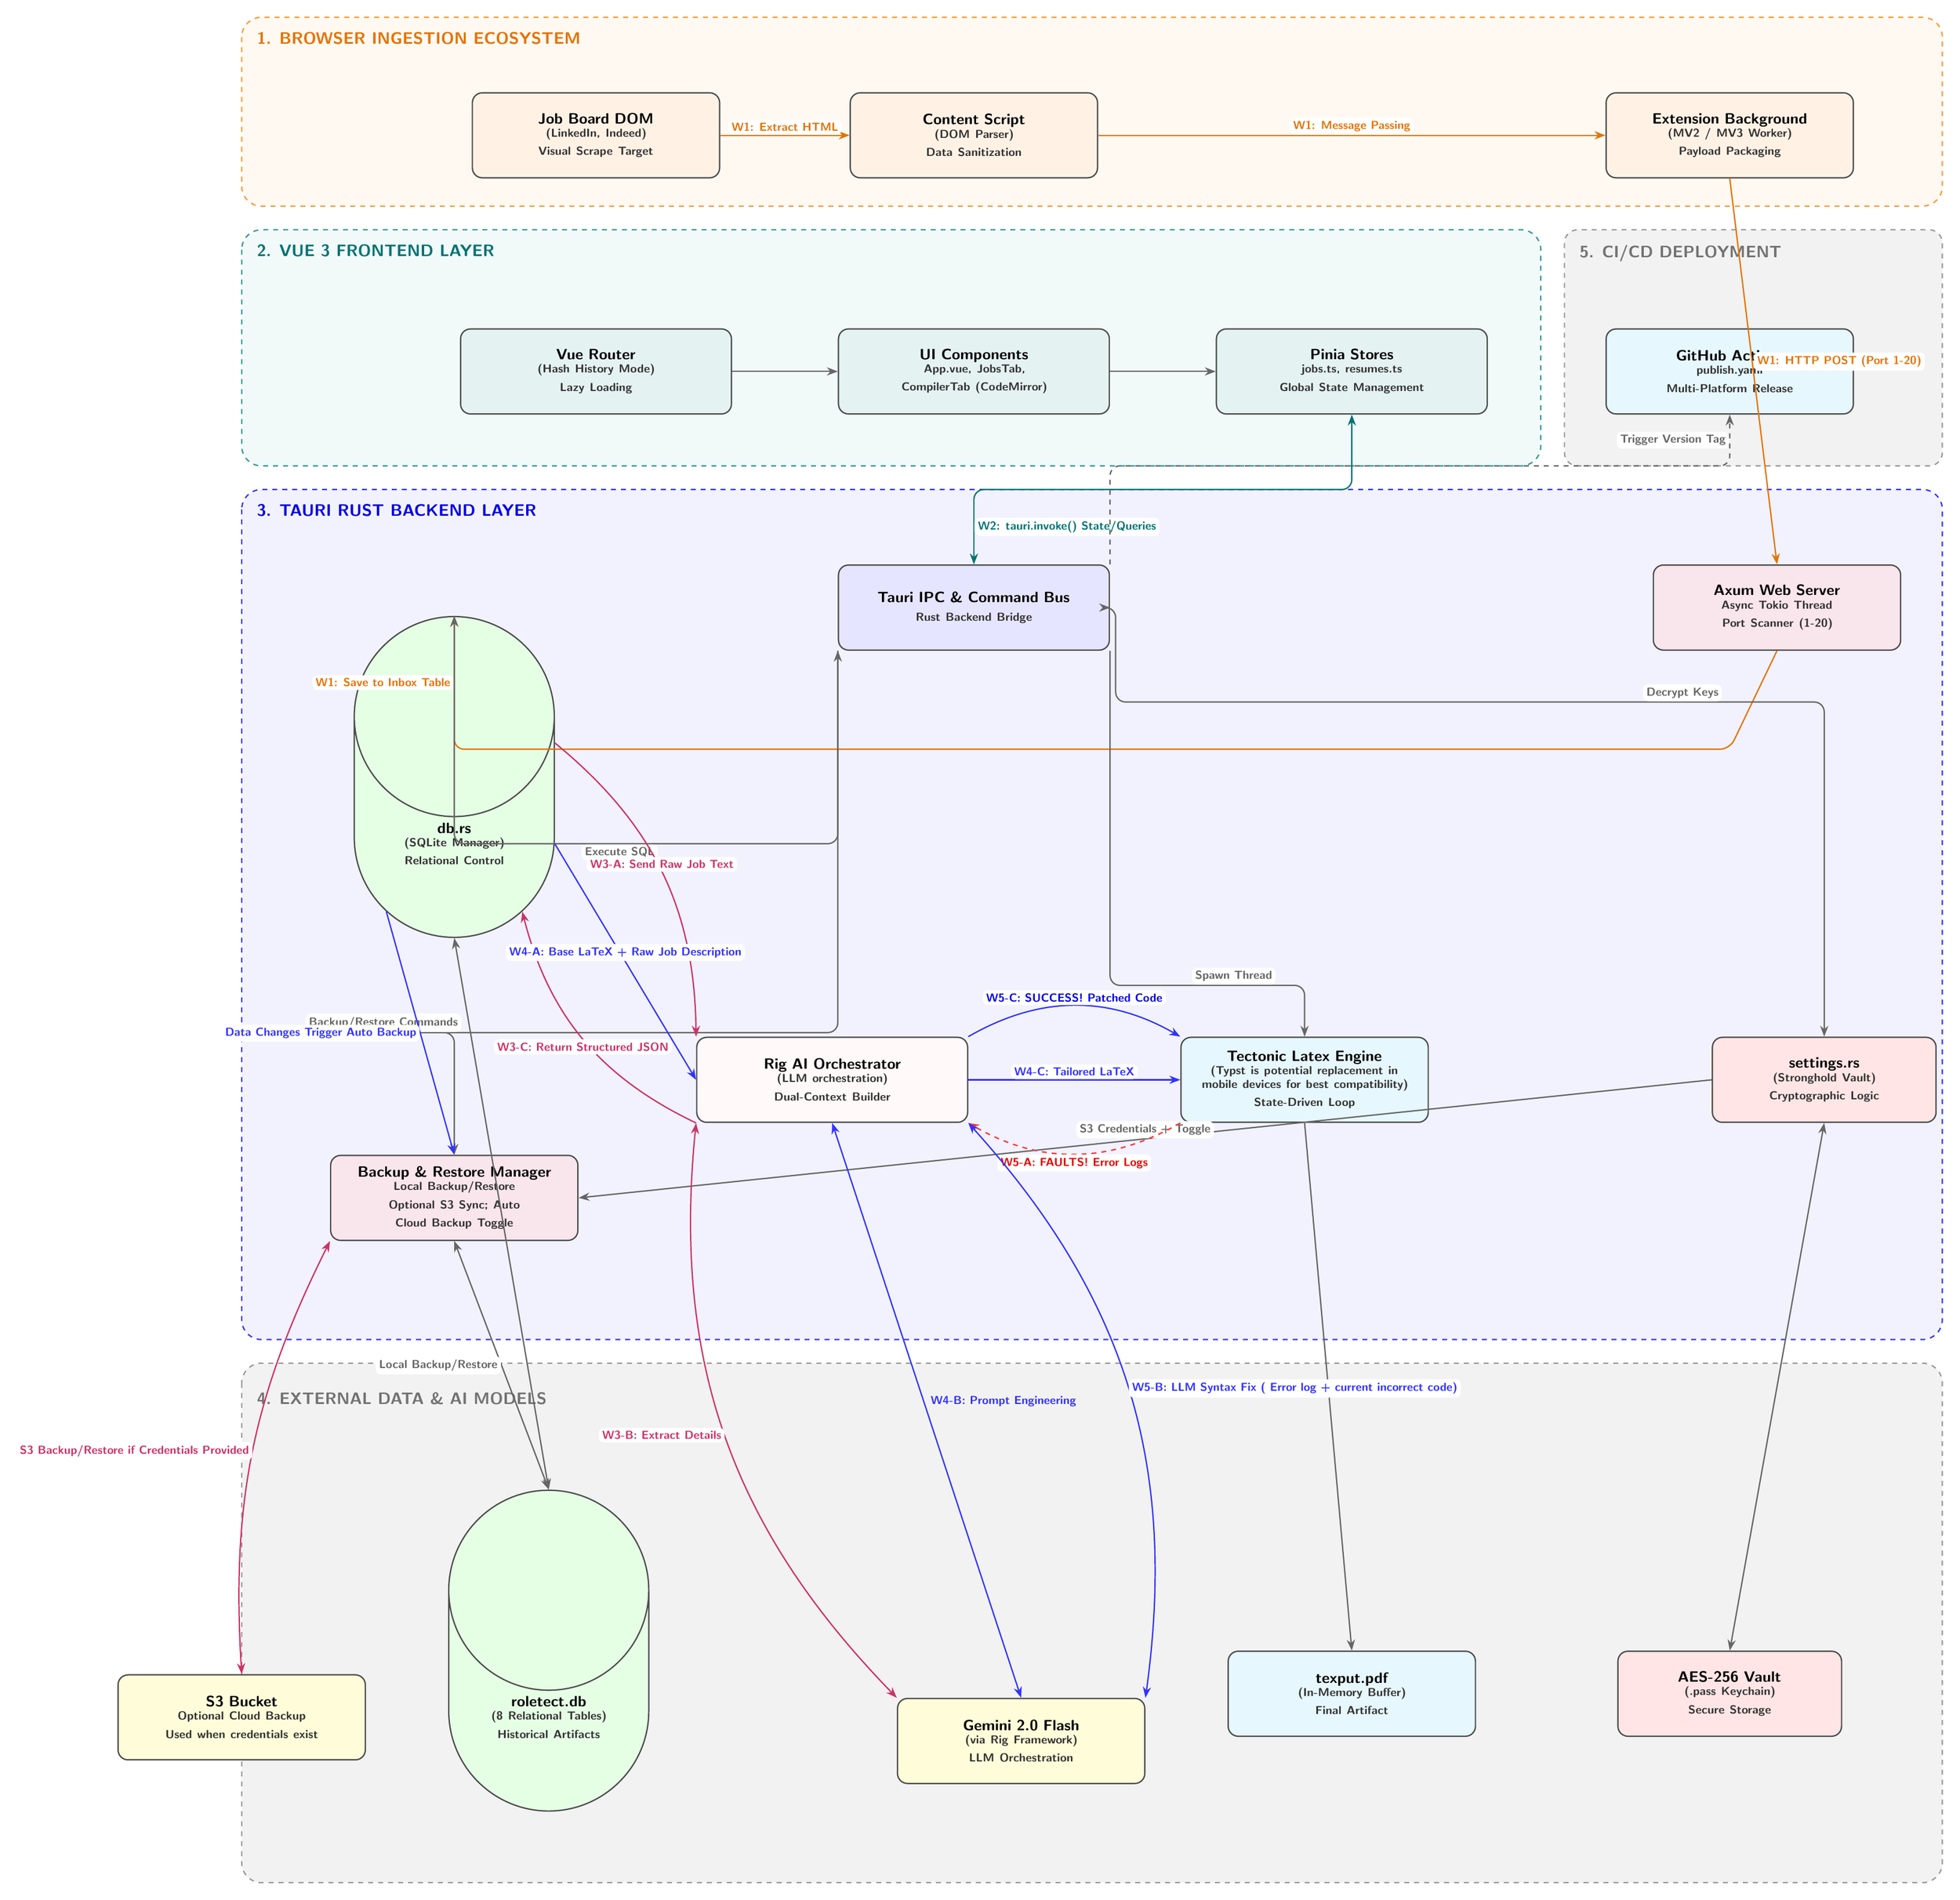
\begin{tikzpicture}[
    auto,
    >=Stealth,
    % Component Styles
    box/.style={draw=black!70, rectangle, rounded corners=6pt, align=center, minimum height=1.8cm, font=\small\sffamily, thick},
    extbox/.style={box, fill=orange!10, text width=5cm},
    uibox/.style={box, fill=teal!10, text width=5.5cm},
    corebox/.style={box, fill=blue!10, text width=5.5cm},
    serverbox/.style={box, fill=purple!10, text width=5cm},
    dbbox/.style={draw=black!70, cylinder, shape border rotate=90, fill=green!10, text width=4cm, align=center, minimum height=2cm, font=\small\sffamily, thick},
    secbox/.style={box, fill=red!10, text width=4.5cm},
    aibox/.style={box, fill=pink!10, text width=5.5cm},
    compbox/.style={box, fill=cyan!10, text width=5cm},
    llmbox/.style={box, fill=yellow!15, text width=5cm},
    % Text Styles
    titlefont/.style={font=\bfseries\sffamily\small},
    descfont/.style={font=\scriptsize\sffamily\color{black!80}},
    lbl/.style={font=\scriptsize\sffamily\bfseries, fill=white, inner sep=2pt, rounded corners=3pt},
    % Workflow Line Styles
    w1/.style={->, thick, color=orange!90!black, rounded corners=6pt},
    w2/.style={<->, thick, color=teal!90!black, rounded corners=6pt},
    w3/.style={->, thick, color=purple!80, rounded corners=6pt},
    w4/.style={->, thick, color=blue!80, rounded corners=6pt},
    w5/.style={->, thick, dashed, color=red!80, rounded corners=6pt},
    standard/.style={->, thick, color=black!60, rounded corners=6pt},
    bistandard/.style={<->, thick, color=black!60, rounded corners=6pt}
]

    % --- BACKGROUND LAYER GROUPS ---
    \draw[dashed, fill=orange!5, draw=orange!80, thick, rounded corners=12pt] (-7.5, 2.5) rectangle (28.5, -1.5);
    \node[anchor=north west, font=\bfseries\sffamily, color=orange!90!black] at (-7.3, 2.3) {1. BROWSER INGESTION ECOSYSTEM};

    \draw[dashed, fill=teal!5, draw=teal!80, thick, rounded corners=12pt] (-7.5, -2.0) rectangle (20.0, -7.0);
    \node[anchor=north west, font=\bfseries\sffamily, color=teal!90!black] at (-7.3, -2.2) {2. VUE 3 FRONTEND LAYER};

    \draw[dashed, fill=gray!10, draw=gray!80, thick, rounded corners=8pt] (20.5, -2.0) rectangle (28.5, -7.0);
    \node[anchor=north west, font=\bfseries\sffamily, color=gray!90!black] at (20.7, -2.2) {5. CI/CD DEPLOYMENT};

    \draw[dashed, fill=blue!5, draw=blue!80, thick, rounded corners=12pt] (-7.5, -7.5) rectangle (28.5, -25.5);
    \node[anchor=north west, font=\bfseries\sffamily, color=blue!90!black] at (-7.3, -7.7) {3. TAURI RUST BACKEND LAYER};

    \draw[dashed, fill=gray!10, draw=gray!80, thick, rounded corners=12pt] (-7.5, -26.0) rectangle (28.5, -37.0);
    \node[anchor=north west, font=\bfseries\sffamily, color=gray!90!black] at (-7.3, -26.5) {4. EXTERNAL DATA \& AI MODELS};

    % --- NODES ---
    % Layer 1
    \node [extbox]  at (0, 0) (DOM) {\titlefont Job Board DOM \\ \descfont (LinkedIn, Indeed) \\ \descfont Visual Scrape Target};
    \node [extbox]  at (8, 0) (CS) {\titlefont Content Script \\ \descfont (DOM Parser) \\ \descfont Data Sanitization};
    \node [extbox]  at (24, 0) (BG) {\titlefont Extension Background \\ \descfont (MV2 / MV3 Worker) \\ \descfont Payload Packaging};

    % Layer 2
    \node [uibox]   at (0, -5) (Router) {\titlefont Vue Router \\ \descfont (Hash History Mode) \\ \descfont Lazy Loading};
    \node [uibox]   at (8, -5) (Views) {\titlefont UI Components \\ \descfont App.vue, JobsTab, \\ \descfont CompilerTab (CodeMirror)};
    \node [uibox]   at (16, -5) (Pinia) {\titlefont Pinia Stores \\ \descfont jobs.ts, resumes.ts \\ \descfont Global State Management};

    % Layer 5 (CI/CD positioned here to fit logically)
    \node [compbox] at (24, -5) (CICD) {\titlefont GitHub Actions \\ \descfont publish.yaml \\ \descfont Multi-Platform Release};

    % Layer 3
    \node [corebox] at (8, -10) (TauriIPC) {\titlefont Tauri IPC \& Command Bus \\ \descfont Rust Backend Bridge};
    \node [serverbox] at (25, -10) (Axum) {\titlefont Axum Web Server \\ \descfont Async Tokio Thread \\ \descfont Port Scanner (1-20)};

    \node [dbbox]   at (-3, -15) (RustDB) {\titlefont db.rs \\ \descfont (SQLite Manager) \\ \descfont Relational Control};
    \node [aibox]   at (5, -20) (RustAI) {\titlefont Rig AI Orchestrator \\ \descfont (LLM orchestration) \\ \descfont Dual-Context Builder};
    \node [compbox] at (15, -20) (RustTex) {\titlefont Tectonic Latex Engine \\ \descfont (Typst is potential replacement in mobile devices for best compatibility) \\ \descfont State-Driven Loop};
    \node [secbox]  at (26, -20) (RustSec) {\titlefont settings.rs \\ \descfont (Stronghold Vault) \\ \descfont Cryptographic Logic};
    \node [serverbox] at (-3, -22.5) (Backup) {\titlefont Backup \& Restore Manager \\ \descfont Local Backup/Restore \\ \descfont Optional S3 Sync; Auto Cloud Backup Toggle};

    % Layer 4
    \node [dbbox]   at (-1, -33.5) (SQLite) {\titlefont roletect.db \\ \descfont (8 Relational Tables) \\ \descfont Historical Artifacts};
    \node [llmbox]  at (9, -34) (Gemini) {\titlefont Gemini 2.0 Flash \\ \descfont (via Rig Framework) \\ \descfont LLM Orchestration};
    \node [compbox] at (16, -33) (PDF) {\titlefont texput.pdf \\ \descfont (In-Memory Buffer) \\ \descfont Final Artifact};
    \node [secbox]  at (24, -33) (Vault) {\titlefont AES-256 Vault \\ \descfont (.pass Keychain) \\ \descfont Secure Storage};
    \node [llmbox]  at (-7.5, -33.5) (S3) {\titlefont S3 Bucket \\ \descfont Optional Cloud Backup \\ \descfont Used when credentials exist};

    % --- W1: INGESTION WORKFLOW ---
    \draw [w1] (DOM.east) -- node[lbl] {W1: Extract HTML} (CS.west);
    \draw [w1] (CS.east) -- node[lbl] {W1: Message Passing} (BG.west);
    \draw [w1] (BG.south) -- node[lbl] {W1: HTTP POST (Port 1-20)} (Axum.north);
    \draw [w1] (Axum.south) -- (24, -13) -| node[lbl, near end] {W1: Save to Inbox Table} (RustDB.north);

    % --- W2: FRONTEND TO BACKEND ---
    \draw [standard] (Router.east) -- (Views.west);
    \draw [standard] (Views.east) -- (Pinia.west);
    \draw [w2] (Pinia.south) -- (16, -7.5) -| node[lbl, near end] {W2: tauri.invoke() State/Queries} (TauriIPC.north);

    % --- BACKEND STANDARD ROUTING ---
    \draw [bistandard] (TauriIPC.south west) |- (4, -15) -| node[lbl, near start] {Execute SQL} (RustDB.north);
    \draw [standard] (TauriIPC.south west) |- (-6, -19) -| node[lbl, near start] {Backup/Restore Commands} (Backup.north);
    \draw [standard] (TauriIPC.south east) |- (12, -18) -| node[lbl, near start] {Spawn Thread} (RustTex.north);
    \draw [bistandard] (TauriIPC.east) -- (11, -10) |- (20, -12) -| node[lbl, near start] {Decrypt Keys} (RustSec.north);
    \draw [standard, dashed] (TauriIPC.north east) |- (12, -7) -| node[lbl, near end] {Trigger Version Tag} (CICD.south);

    % --- EXTERNAL LINKS ---
    \draw [bistandard] (RustDB.south) -- (SQLite.north);
    \draw [w4] (RustDB.south west) -- node[lbl, left] {Data Changes Trigger Auto Backup} (Backup.north);
    \draw [bistandard] (Backup.south) -- node[lbl, left] {Local Backup/Restore} (SQLite.north);
    \draw [w3, <->] (Backup.south west) to[bend right=15] node[lbl, left] {S3 Backup/Restore if Credentials Provided} (S3.north);
    \draw [standard] (RustSec.west) -- node[lbl, above] {S3 Credentials + Toggle} (Backup.east);
    \draw [standard] (RustTex.south) -- (PDF.north);
    \draw [bistandard] (RustSec.south) -- (Vault.north);

    % --- W3: AI PARSING WORKFLOW ---
    \draw [w3] (RustDB.north east) to[bend left=25] node[lbl, above] {W3-A: Send Raw Job Text} (RustAI.north west);
    \draw [w3, <->] (RustAI.south west) to[bend right=25] node[lbl, left] {W3-B: Extract Details} (Gemini.north west);
    \draw [w3] (RustAI.south west) to[bend left=25] node[lbl, below] {W3-C: Return Structured JSON} (RustDB.south east);

    % --- W4: AI TAILORING WORKFLOW ---
    \draw [w4] (RustDB.east) -- node[lbl, above] {W4-A: Base LaTeX + Raw Job Description} (RustAI.west);
    \draw [w4, <->] (RustAI.south) -- node[lbl, fill=none] {W4-B: Prompt Engineering} (Gemini.north);
    \draw [w4] (RustAI.east) -- node[lbl, above] {W4-C: Tailored LaTeX} (RustTex.west);

    % --- W5: SELF-HEALING LOOP ---
    \draw [w5] (RustTex.south west) to[bend left=30] node[lbl, below, text=red!90!black] {W5-A: FAULTS! Error Logs} (RustAI.south east);
    \draw [w4, <->] (RustAI.south east) to[bend left=25] node[lbl, right] {W5-B: LLM Syntax Fix ( Error log + current incorrect code)} (Gemini.north east);
    \draw [w4] (RustAI.north east) to[bend left=30] node[lbl, above, text=blue!90!black] {W5-C: SUCCESS! Patched Code} (RustTex.north west);

\end{tikzpicture}
}
\end{center}
\vspace*{0.5cm}




















% =========================================================================
% PAGE 3: INGESTION \& ASYNC MICRO-SERVER
% =========================================================================
\section{Technical Architecture \& Ingestion Subsystems}
RoleTect is a local-first, privacy-centric suite built on Tauri v2, Axum. To eliminate the fragility of standard input polling, the desktop core transforms the host machine into an isolated micro-web ingress gateway using a custom asynchronous server architecture.

\subsection{The Local Asynchronous Micro-Server Pipeline}
During bootstrapping, the core Tauri binary spins up a dedicated multi-threaded worker space powered by the \texttt{tokio::runtime} async environment, initializing a high-performance, lightweight Axum web router. This local node functions as a non-blocking receiver for incoming job descriptions captured from the browser.

 ncoming payloads are instantly validated, sanitized, and pushed securely into a local SQLite staging layer, surfacing inside the application's ``Inbox Tab.''

\subsection{Dynamic Socket Allocation and Collision Mitigation}
Binding services to rigid static addresses (e.g., \url{localhost:8080}) creates port collision faults if another background process occupies that socket. RoleTect resolves this liability by implementing an intelligent, socket negotiation protocol across an active port:
\begin{equation}
\text{Port\_Pool} = \{ P_{\text{start}}, P_{\text{start}} + 1, P_{\text{start}} + 2, \dots, P_{\text{start}} + 19..... \}
\end{equation}
On initialization, the Tokio runtime probes each sequential port configuration. The first unassigned socket flagged by the OS is instantly captured and bound to the Axum engine. \textbf{This dynamic address is then saved to the local user profile, removing manual port debugging or administrative configuration.}

\subsection{Dual DOM Ingestion: Visual Mouse-Selector Mode \& Manual attribute based}
The RoleTect Helper Extension streamlines data collection via a visual element selector. When activating ``Selector Mode,'' the extension treats the live webpage DOM as an interactive map, drawing bounding boxes over content structures as the user hovers. Upon clicking a section, the extension executes a rapid script:
\begin{enumerate}
    \item Isolates the unique DOM ID tags or parent CSS class names of the targeted area.
    \item Recursively crawls underlying child nodes to extract raw textual data blocks.
    \item Strips out dynamic script components, ad tracking metrics, and volatile inline styles.
    \item Checks the active port generated by the desktop core and fires an \texttt{HTTP POST} payload directly to \texttt{localhost:[Dynamic\_Port]}.
\end{enumerate}

\subsection{Ecosystem Adaptability: Local vs. Cloud Targets (In future)}
\textbf{The extention connection manager is engineered to handle variable routing matrices}. Beyond native local discovery over the dynamic localhost pipeline, the configuration portal accommodates custom remote endpoints. Advanced users opting to deploy their Axum framework core on a private Virtual Private Server (VPS) can replace the default localhost loop with their secure cloud domain, bridging local-first sovereignty with scalable cloud configurations.


% ==========================================
% PAGE 4: PROCESSING ENGINES & MOBILE ARCHITECTURE
% ==========================================

\vspace{30mm}


\section{Processing Engines \& Cross-Platform Architecture}
RoleTect decouples document generation from corporate SaaS networks by integrating a local-first orchestration layer alongside an embedded cross-platform compilation engine. This architecture guarantees document rendering viability across multiple os.






\subsection{The Multi-Provider AI Architecture via Rig}
Rather than binding to a single AI vendor, RoleTect deploys the Rust-native \textbf{Rig Framework} as a type-safe, model-agnostic abstraction layer. Candidates connect their preferred endpoint through the security panel, controlling resource allocation on a strict pay-per-token basis:
\begin{itemize}
    \item \textbf{Commercial \& Enterprise Cloud:} Seamless connectivity to OpenAI, Anthropic, Gemini, and encrypted AWS Bedrock nodes.
    \item \textbf{Custom \& Regional Engines:} Base URL parameter mapping for specialized deep-reasoning layers like DeepSeek or Kimi.
    \item \textbf{Air-Gapped Privacy Nodes:} Full integration with local \texttt{Ollama} daemons to execute open-weights models (e.g., Llama 3) entirely on-device with zero network footprint and zero token fees.
\end{itemize}

\textbf{The Rig framework handles dual-context generation loops. The raw text payload (\texttt{raw\_job\_content}) is analyzed alongside structural system prompts. Rig requests a structured JSON payload containing tracking metadata attributes }(\texttt{company\_name}, \texttt{job\_title}, \texttt{target\_salary}) while maintaining the core resume text within volatile operational memory.














\subsection{Local Tectonic Typesetting and Self-Healing Error Loops}
On our systems, RoleTect links natively to the \textbf{Tectonic} engine—an advanced, cached typesetting ecosystem derived from \textbf{XeTeX}. Following an initial online bootstrapping phase that downloads and stores standard macros and style templates, all document processing executes completely offline within sub-millisecond compile loops.

If the LLM generates syntactically broken \LaTeX{} markup, RoleTect mitigates system faults through a state-driven self-healing recovery routine:
\begin{equation}
\text{State}_{\text{error}} \longrightarrow \text{Rig}(\text{Code}_{\text{broken}} + \text{Log}_{\text{tectonic}}) \longrightarrow \text{Code}_{\text{healed}} \longrightarrow \text{Compile}_{\text{retry}}
\end{equation}
The application intercepts the console compilation error output, dynamically logging it to the \texttt{resume\_errors} or \texttt{coverletter\_errors} fields within the SQLite schema. Instead of halting, the interface passes the \textbf{broken code and the precise compilation log} back to the \textbf{Rig framework}. The model outputs a structural data, executes a background re-compilation, and—upon a verified successful render—wipes the error database entry clean.

\subsection{Cross-Platform Mobile Strategy: The Tauri v2 Typst  (Future implementation)}
To scale the platform across mobile target infrastructures, RoleTect will leverages the unified runtime properties of the \textbf{Tauri v2} core ecosystem, enabling successful deployment setups like verified Android APK binaries.

Because executing \textbf{multi-gigabyte XeTeX} compilation layers via Tectonic introduces significant hardware boundaries on \textbf{ARM-based mobile} devices, RoleTect plans to employ a highly efficient \textbf{dual-engine} rendering strategy. On mobile form factors, the document compilation workflow transitions seamlessly onto a native \textbf{Typst} processing core. Typst's streamlined syntax requires far lower system footprints than traditional \LaTeX{}, providing an ultra-fast, linear code environment that enables the Rig framework to generate error-free professional documents on mobile devices without thermal or processing performance penalties.




\vspace{10mm}



% ==========================================
% PAGE 5: HYBRID CLOUD ROADMAP & HACKATHON CONCLUSION
% ==========================================

\section{Hybrid Cloud Strategy (Clould VPS is Ongoing) \& Performance Analysis}

\subsection{Current Architectural Limitations \& The Cloud Pathway}
While a local-first architecture effectively secures a candidate's data sovereignty during the document drafting phase, tracking real-world application statuses presents a structural limitation: \textbf{local systems cannot detect external recruiter interactions once a file leaves the host machine}.

To resolve this operational boundary without sacrificing user privacy, RoleTect has planned an elegant hybrid cloud expansion pathway. The system maps its internal database schema onto a custom-deployable cloud instance, allowing high-volume users to host an \textbf{identical web-compiled Axum backend} paired with a high-performance Next.js interface on a \textbf{private Virtual Private Server (VPS)}.

\subsection{The Next.js + Axum Cloud Analytics Vector}
This VPS configuration \textbf{enables secure, isolated event-tracking hooks}. When a resume or cover letter is deployed via the cloud node, the system \textbf{injects transparent, unique parameters into outbound communication strings}.

This infrastructure allows the user to:
\begin{itemize}
    \item Log exactly when a PDF document link is opened.
    \item Verify email delivery statuses within a private, dedicated dashboard.
    \item Completely eliminate reliance on commercial marketing software that harvests applicant behaviors.
\end{itemize}

\subsection{Data Management: Backup, Restore, Synchronization \& Staging}
To maintain seamless data consistency across local desktop environments, mobile devices, and private VPS clusters or \textbf{Cloud S3}, RoleTect implements a robust physical storage configuration for syncing SQLite databases via two primary mechanisms:
\begin{itemize}
    \item \textbf{The Overwrite Restore Routine:} Replaces the target device's active database file entirely with a clean, timestamped snapshot from the master machine.
    \item \textbf{The Temporal Merge Routine:} Analyzes internal transaction logs chronologically, stitching unique job rows and document variants from both databases together without risk of data corruption.
\end{itemize}

Furthermore, incoming data from the browser extension enters a dedicated \texttt{Inbox Staging Table}. This acts as an isolated buffer, \textbf{preventing unparsed or raw data fragments from cluttering active application vaults} until the user explicitly prompts the system to execute a Rig compilation loop.

\subsection{Future Plan \& Development Roadmap}
Building upon this hybrid foundation, the upcoming phase of the development roadmap focuses on optimizing the automation of these distributed nodes. Future iterations will introduce automated zero-downtime synchronization triggers and pre-configured Docker environments to make the private VPS deployment friction-free for non-technical users.

\subsection{Architectural Matrix \& Optimization Breakdown}
Operating a secure, completely air-gapped system introduces explicit environment setup dependencies, initial network-bound package latency, and hardware platform constraints. Table 3 outlines these current core limitations, the engineering remedies active in the production codebase, and the long-term hybrid cloud execution roadmap.




\subsection{Instant Execution Capabilities Matrix}
To maximize operational efficiency, RoleTect does not force users through a long onboarding loop. The platform bifurcates its capability access based on credential provisioning, allowing immediate deployment of local workspaces prior to setting up cloud or model connectivity.

\begin{table}[h]
\centering
\caption{Feature Access Thresholds based on User Configuration}
\vspace{2mm}
\small
\begin{tabular}{p{7.2cm}p{7.2cm}}
\toprule
\textbf{Unlocked Instantly (50MB Clean Install)} & \textbf{Unlocked Post-Credential Setup (API + S3)} \\
\midrule
$\bullet$ \textbf{Zero-Setup \LaTeX{} Workspace} runs fully offline after using embedded distribution caches for first time that downloads most used 85 packages \& cache it. & $\bullet$ \textbf{Visual Raw-to-Vault Processing} automatically structuralizes raw text via LLM parse chains. \\
\addlinespace
$\bullet$ \textbf{Full Markdown IDE} executes native real-time document rendering with no external engines. & $\bullet$ \textbf{Contextual Resume Tailoring} drives precision profile modification using targeted job parameters. \\
\addlinespace
$\bullet$ \textbf{Vector Diagram Studio} renders high-fidelity Mermaid architecture charts with up to 16K export resolution. & $\bullet$ \textbf{Self-Healing Compile Loops} automatically ingest Tectonic syntax logs to auto-fix code errors. \\
\addlinespace
$\bullet$ \textbf{ Data Ingestion (Browser Data Ingestion Extention)} sends clean, stripped \texttt{raw\_job\_content} directly into the application Inbox. & $\bullet$ \textbf{Durability Cloud Backups} push localized database snapshot records seamlessly to secure S3 storage. \\
\bottomrule
\end{tabular}
\end{table}


\begin{table}[h]
\centering
\caption{Limitations, Native Fixes, and Architecture Roadmap}
\vspace{2mm}
\small
\begin{tabular}{p{4.2cm}p{5.2cm}p{5.2cm}}
\toprule
\textbf{Current Technical Limitation} & \textbf{Active Engineering Solution} & \textbf{Future Hybrid Roadmap Plan} \\
\midrule
\textbf{Infrastructure Configuration:} Users must manually input provider API keys, provision S3 access keys, bucket key for cloud backup or AI orchestration. & Localized snapshot backup subsystem operates implicitly out-of-the-box, need \textbf{S3 credentials for cloud backup}, ensuring total file durability if local host storage remains intact. &Automated lifecycle policies that securely sync local snapshot deltas to the configured cloud object storage bucket at scheduled intervals, providing automated off-site disaster recovery.\\
\addlinespace
\textbf{Initial Package Latency:} Tectonic must fetch and build layout macro files online during initial setup, generating a 1--2 minute first-compile bottleneck. & Pre-cached baseline templates containing the \textbf{85 most common packages} can be built once natively within the IDE, dropping \textbf{offline renders to 10--40 seconds}. & Automated first-compile hydration routines that programmatically pull and cache core macro distributions upon initial application initialization. \\
\addlinespace
\textbf{Hardware Target Matching:} Non-technical candidates must explicitly locate and fetch the exact binary package matching their specific OS and hardware architecture. & Granular documentation profiles and clear, deterministic cross-compilation deployment guides are actively hosted on software release portals. & Unified cross-platform download portal featuring automatic web-based user agent detection and continuous background package updating. \\
\bottomrule
\end{tabular}
\end{table}

\subsection{System Execution Context}
As demonstrated by this architectural trade-off ledger, the processing velocity of the document generation engine relies tightly on host CPU capabilities. While modern consumer hardware possess highly efficient processing power to handle these compilation threads with minimal friction, low-power microarchitectures require this optimization structure to guarantee execution fluidity. \textbf{By keeping data localized yet exposing an upgrade path to private analytics instances, RoleTect balances data privacy against data tracking utility.}

\end{document}
